\documentclass[a4paper,12pt]{article}
\usepackage[utf8]{inputenc}
% Resten af pakkerne
\usepackage[english]{babel}
\usepackage{csquotes}
\usepackage{float}
\usepackage{flafter}
\usepackage{graphicx}
\usepackage{setspace}
\usepackage{enumitem}
\usepackage{multirow}
\usepackage{lmodern}
\usepackage{amssymb,amsmath}
\usepackage{ifxetex,ifluatex}
\usepackage[font=small,labelfont=bf]{caption}
\usepackage{lscape}
\usepackage{xargs}
\usepackage{tabularx}
\usepackage{comment}
\usepackage{pdfpages}
\usepackage{xcolor}
\usepackage{amssymb} 
\usepackage[normalem]{ulem}

\usepackage{listings}

\usepackage{ragged2e}

\definecolor{mygreen}{rgb}{0,0.6,0}

\lstnewenvironment{code}[1][]%
{
   \noindent
   \minipage{\linewidth} 
   \vspace{0.5\baselineskip}
   \lstset{language=java, basicstyle=\ttfamily\footnotesize,frame=single,#1}}
{\endminipage}


\lstset{
    stringstyle=\color{mygreen},            % changing string colour to green
    frame=single,                           % adds a frame around the code
    language=Java,                          % the language of the code
    breaklines=true,                        % sets automatic line breaking
    basicstyle=\small,                      % the size of the fonts that are used for the code
    keywordstyle=\color{blue},              % keyword style
    morekeywords={var, UUID, ROLE, EMAIL},  % if you want to add more keywords to the set
    numbers=left,                           % % where to put the line-numbers; possible values are (none, left, right)
    numberstyle=\small,                     % the style that is used for the line-numbers
    commentstyle=\color{mygreen},           % comment style
    captionpos=b,                           % sets the caption-position to bottom
    showstringspaces=false,                  % removes spaces in string
    inputencoding=utf8,
    extendedchars=true,
}

\lstset{literate=%
{æ}{{\ae}}1
{å}{{\aa}}1
{ø}{{\o}}1
{Æ}{{\AE}}1
{Å}{{\AA}}1
{Ø}{{\O}}1
}

% Use for lstlisting formation caption
% \captionsetup[lstlisting]{ format=listing, labelfont=white, textfont=white, singlelinecheck=false, margin=0pt, font={bf,footnotesize}}

% \usepackage[
% backend=biber,
% style=alphabetic,
% sorting=ynt
% ]{biblatex}
% \addbibresource{appendices/bibliography.bib}

% \title{Bibliography management: \texttt{biblatex} package}
% \author{Overleaf}
% \date{ }

\usepackage{ifthen}

\usepackage{xcolor}
% \usepackage{csvsimple}
\usepackage{longtable}

% Margin
\usepackage{geometry}
\geometry{a4paper,  total={170mm,250mm},
 left=20mm,
 top=25mm}


% New Commands
\newcommand\myworries[1]{\textcolor{red}{#1}} 
\newcommand{\myparagraph}[1]{\paragraph{#1}\mbox{}\\}


% Needs to be the last package included
\usepackage{hyperref}
\hypersetup{
    colorlinks=true,
    linkcolor=black,
    filecolor=magenta,      
    urlcolor=blue,
    citecolor=black,
}

\setlength\parindent{0pt} % Removes indent

\begin{document}
    % Fjerner side tal
    \pagenumbering{gobble}
    \renewcommand{\thesection}{\Roman{section}} 
    \renewcommand{\thesubsection}{\thesection.\Roman{subsection}}
    % Forside
    \begin{titlepage}
\begin{center}
% Title
{ \LARGE \bfseries Bierproductie \\[0.4cm]}
A management system for brewing machines
\begin{figure}[H]
\centering 
\includegraphics[scale=0.5]{images/system_drawing.png}
\label{figure:bierproductie_system}
\end{figure}

Bachelor of Engineering, Software Technology\\
\vspace{2mm}
Semesterproject 3. semester, ST3-PRO\\
\vspace{2mm}
\textbf{Project Period:} 31.08.2020 - 19.12.2020 \\
\vspace{2mm}
\textbf{Hand in date:} 19.12.2020 \\

\vspace{7mm}

\textbf{Group 06:} \\
\vspace{2mm}
Jakob Rasmussen, jakra19@student.sdu.dk \\
\vspace{2mm}
Kenneth M. Christiansen kechr19@student.sdu.dk \\
\vspace{2mm}
Kevin K. M. Petersen, kepet19@student.sdu.dk \\
\vspace{2mm}
Kristian N. Jakobsen, kjako19@student.sdu.dk \\
\vspace{2mm}
Simon Jørgensen, sijo819@student.sdu.dk \\

\vspace{7mm}

\textbf{Supervisor:} Parisa Niloofar, parni@mmmi.sdu.dk \\

% Bottom of page
\vfill

University of Southern Denmark \\
The Faculty of Engineering \\
The Mærsk Mc-Kinney Møller Institute \\
Campusvej 55, 5230 Odense M 

\end{center}
\end{titlepage}

    \newpage
    
    % Titelblad 
    % \begin{tabular}{@{}l l} 
\textbf{Title:} & Bierproductie \\
& \\
\textbf{Institution:} & University of Southern Denmark \\
& The Faculty of Engineering, The Mærsk Mc-Kinney Møller Institute \\
& Campusvej 55, 5230 Odense M \\
& \\
\textbf{Education:} & Bachelor of Engineering, Software Technology\\
& \\
\textbf{Semester:} & 3. Semester \\
& \\
\textbf{Course Title:} & Industrial 4.0 cyber-physical software systems \\
& \\
\textbf{Internal Course Code:} & ST3-PRO \\
& \\
\textbf{Project Period:} &  31.08.2020 - 19.12.2020\\
& \\
\textbf{ECTS:} & 10 ECTS\\
& \\
\textbf{Supervisor:} & Parisa Niloofar\\
& \\
\textbf{Project group:} & 06\\
& \\

\\
\end{tabular}

% VARIABLES
\newcounter{PROD}
\setcounter{PROD} {1}

%%%%


% Jakob Jakob Jakob Jakob Jakob Jakob Jakob Jakob Jakob Jakob Jakob
\ifnum \value{PROD}=1
    
\includegraphics[scale=0.07]{images/signatures/signatureJR.jpg}
    \vspace{-9.5mm}
\fi
\par\rule{\textwidth}{0.4pt}

Jakob Rasmussen, jakra19@student.sdu.dk\\
% -end- -end- -end -end -end- -end- -end -end -end- -end- -end -end -end-

% Kenneth Kenneth Kenneth Kenneth Kenneth Kenneth Kenneth Kenneth Kenneth

\ifnum \value{PROD}=1
    
\includegraphics[scale=0.3]{images/signatures/signature_kechr19.PNG}
    \vspace{-5mm}
\fi
\par\rule{\textwidth}{0.4pt}

Kenneth M. Christiansen, kechr19@student.sdu.dk\\
\vspace{3.5mm}
% -end- -end- -end -end -end- -end- -end -end -end- -end- -end -end -end-

% KEVIN KEVIN KEVIN KEVIN KEVIN KEVIN Kevin Kevin Kevin Kevin Kevin Kevin
\vspace{-6.5mm}

\ifnum \value{PROD}=1
    
\includegraphics[scale=0.3]{images/signatures/signature_kepet19.png}
    \vspace{-8mm}
\fi
\par\rule{\textwidth}{0.4pt}

Kevin K. M. Petersen, kepet19@student.sdu.dk
% -end- -end- -end -end -end- -end- -end -end -end- -end- -end -end -end-

% Kristian Kristian Kristian Kristian Kristian Kristian Kristian

\ifnum \value{PROD}=1
    
\includegraphics[scale=0.04]{images/signatures/signature_kjako19.jpg}
    \vspace{-9.5mm}
\fi
\par\rule{\textwidth}{0.4pt}

Kristian N. Jakobsen, kjako19@student.sdu.dk\\
% -end- -end- -end -end -end- -end- -end -end -end- -end- -end -end -end-

% Simon Simon Simon Simon Simon Simon Simon Simon Simon Simon Simon Simon

\ifnum\value{PROD}=1
    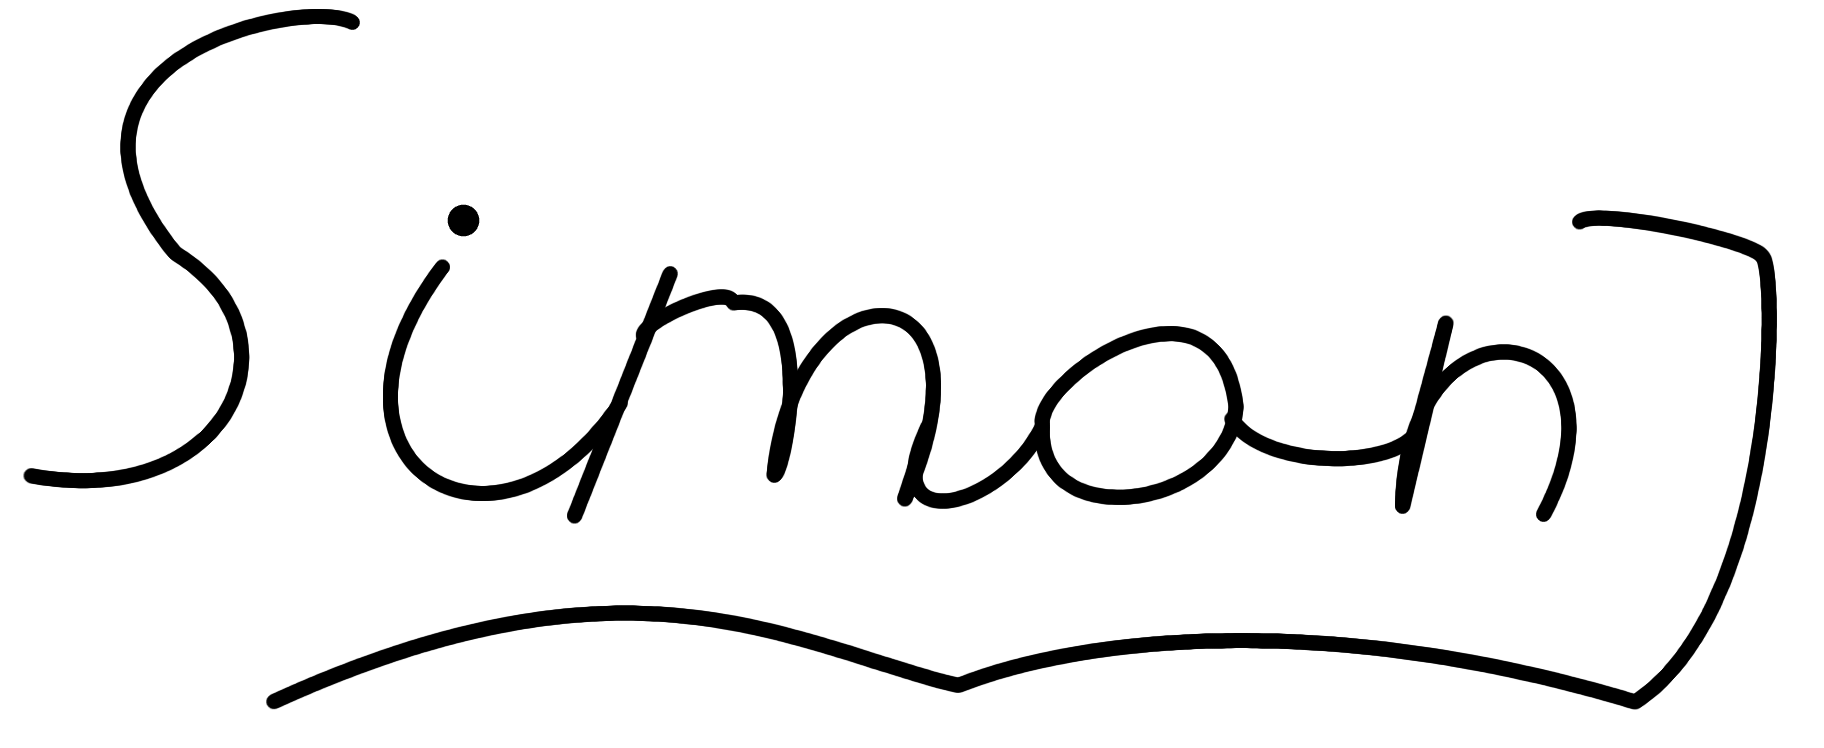
\includegraphics[scale=0.042]{images/signatures/signatureSJ.png}
    \vspace{-3.5mm}
\fi
\par\rule{\textwidth}{0.4pt}

Simon Jørgensen, sijo819@student.sdu.dk\\
% -end- -end- -end -end -end- -end- -end -end -end- -end- -end -end -end-

%Bottom of page
%\vfill

\begin{tabular}{@{}l l}
Pages:      & 21 \myworries{Remember me :)} \\
Appendix:   & 0 \myworries{And me! :)}
\end{tabular}

\vspace{3.5mm}

\begin{footnotesize}

\textbf{By signing this document, each group member confirms that everyone have participated equally to this project, and everyone is thus collectively responsible for the content of the report.}
\end{footnotesize}

    % \newpage

    % % Resume
    % \input{tex/iii_resume}
    % \newpage
    
    % % Forord
    % \input{tex/iv_forord}
    % \newpage

    % % Indholdsfortegnelse
    % \setcounter{tocdepth}{2} % anything below subsection will not be added
    % \input{tex/v_indholdsfortegnelse}
    % \newpage
    
    % % Læsevejledning
    % \input{tex/vi_læsevejledning}
    % \newpage
    
    % \input{tex/vii_redaktionelt}
    % \newpage
    
    % Start counting from this line
    \pagenumbering{arabic}
    \setcounter{page}{1}

    \renewcommand{\thesection}{\arabic{section}} 
    \renewcommand{\thesubsection}{\thesection.\arabic{subsection}}
    \setcounter{section}{0}

    \input{tex/mainpage1.tex}
    %\newpage

    % Introduktion
    % \input{tex/1_indledning}
    % \newpage
    
    % % Metoder & Værktøjer
    % \input{tex/2_1_metoder_og_værktøjer}
    % \newpage
    
    % % Planlægning
    % \input{tex/2_2_planlægning}
    % \newpage
    
    % % Faglige vidensgrundlag
    % \input{tex/3_faglige_vidensgrundlag}
    % \newpage
   
    % % Hovedtekst
    % \input{tex/4_0_hovedtekst}
    % \newpage
    
    % % Diskussion
    % \input{tex/5_diskussion}
    % \newpage
    
    % % Konklusion
    % \input{tex/6_konklusion}
    % \newpage
    
    % % Perspektivering
    % \input{tex/7_perspektivering}
    % \newpage
    
    % % Procesevaluering
    % \input{tex/8_procesevaluering}
    % \newpage

    % % bibliography empty
    % \bibliographystyle{apalike}
    % % \bibliographystyle{alphabetic}
    % % \bibliographystyle{unsrt}
    % \bibliography{appendices/bibliography.bib}
    % % \medskip
    % % \printbibliography
    % \newpage
    
    % % fjerner sidetal
    % \pagenumbering{gobble}
    % % Bilag
    % \appendix % Bruges til bilag, så den laver bilag indholdfortegnelse og overskrifter
    % \input{appendices/bilag.tex}

\end{document}
